% ----- ab hier eigentlicher Inhalt -------------------------------------------

\section{Wegematrix}
\begin{frame}
	\frametitle{Wegematrix I}
	\begin{block}{Darstellung von Relationen}
		So wie die Adjazenzmatrix Relationen zwischen Knoten darstellt, können auch weitere Relationen als Matrix dargestellt werden. Ein Beispiel ist die Wegematrix, die eine Darstellungsform der Erreichbarkeitssrelation
		$E^*=\bigcup^{n-1}_{i=0} E^i $. \\
	\end{block}
	\begin{block}{Für die Wegematrix gilt}
 \begin{displaymath}
 W_{ij}=
	\begin{cases}
		1, & \text{falls es in G einen Pfad von i nach j gibt} \\
		0, & \text{falls es in G keinen Pfad von i nach j gibt}
	\end{cases}
	\end{displaymath}
	\end{block}
\end{frame}

\subsection{Algorithmen}
\begin{frame}
	\frametitle{Aufwand}
	\begin{block}{Zählweise}
		Beim Vergleich verschiedener Algorithmen in Bezug auf den Aufwand, sucht man nach einem Maß für die Anzahl der Rechenoperationen für eine Aufgabe der Größe $n$.
	\end{block}
	\begin{block}{Beispiel} \pause
		Summe aller Zahlen von $1$ bis $n$: \\

			$\sum^n_{i=0} i = $\pause$n*(n+1)/2$

	\end{block}
\end{frame}

\begin{frame}
	\frametitle{Algorithmus I}
% 	\begin{block}{einfacher Algorithmus zur Wegematrix}
% \end{block}

\lstinputlisting{src/tut07_algo1.txt}

\end{frame}

\begin{frame}
	\frametitle{Algorithmus II}
% 	\begin{block}{einfacher Algorithmus zur Wegematrix}
% \end{block}

\lstinputlisting{src/tut07_algo2.txt}

\end{frame}

\begin{frame}
	\frametitle{Algorithmus III}
	\begin{block}{$log_2(n) \cdot n^3$}
		Wir verwenden einen Trick: \pause
		\begin{itemize}
			\item $F=E^0\cup E^1= {Id}_V\cup E$ \pause
			\item dann $F^2 = (E^0\cup E^1)\circ(E^0\cup E^1)= E^0 \cup E^1\cup E^1 \cup E^2= E^0 \cup E^1 \cup E^2$ \pause
			\item und $E^* = \bigcup_{i=0}^{\infty} E^i = \bigcup_{i=0}^{2^m} E^i = F^{2^m}$ \pause
			\item wobei $m=\lceil \log_2 n \rceil$
		\end{itemize}
	\end{block} \pause
\end{frame}

\begin{frame}
	\begin{block}{Aufwandsvergleich}
		Wenn man in einem bestimmten Zeitraum mit dem $n^5$ Algorithmus gerade noch die Problemgröße $n=1000$ schafft: 
	  \begin{itemize}
		  \item Wie große Probleminstanzen schafft man mit dem $n^4$ Algorithmus? \pause
		  \item ... oder mit dem $log_2(n) \cdot n^3$ Algorithmus?
	  \end{itemize}
	\end{block}
\end{frame}

%
%% Der folgende Worsch-Tex will nicht funktionieren:
\begin{frame}
	\frametitle {Wegematrix}
	\begin{columns}
		\column{.5\textwidth}
		\begin{center}
		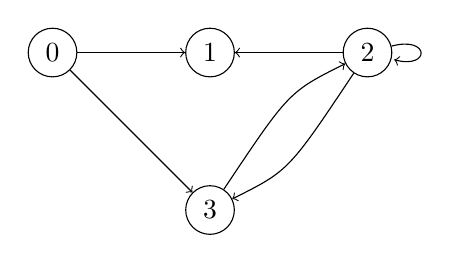
\begin{tikzpicture}
		  \tikzstyle{every node}=[draw,shape=circle];
			\path[fill] (0,0)  node[circle] (0) {0};
			\path[fill] (2,0)  node[circle] (1) {1};
			\path[fill] (4,0)  node[circle] (2) {2};
			\path[fill] (2,-2) node[circle] (3) {3};

			\path[->,draw] (0) -- (1);
			\path[->,draw] (2) -- (1);
			\path[->,draw] (2) edge [loop right] ();
			\path[->,draw] (3) .. controls (3,-0.5) ..  (2);
			\path[->,draw] (2) .. controls (3,-1.5) ..  (3);
			\path[->,draw] (0) -- (3);
		\end{tikzpicture}
		\end{center}
    \column{.5\textwidth}
				$\left(
						\begin{matrix}
							0 & 1 & 0 & 1 \\
							0 & 0 & 0 & 0 \\
							0 & 1 & 1 & 1 \\
							0 & 0 & 1 & 0
						\end{matrix}
				\right)$
	\end{columns}
	\begin{block}{Ihr seid dran...}
		\begin{itemize}
			\item Wie sieht die Wegematrix zum oben gezeigten Graph aus?
			\visible<2->{\item Wie sieht die Wegematrix für eine vollständig mit 1en gefüllte Matrix aus?}
			\visible<3->{\item Wann gilt allgemein $W=A$? Wann gilt $E^1=A$?}
		\end{itemize}
	\end{block}
\end{frame}

\section{Warshall-Algorithmus}
\subsection*{}
\begin{frame}
	\frametitle{Reflexive Transitive Hülle nach Warshall}

	Gegeben sei eine reflexive Relation $\rho$ über einer endlichen Eckenmenge $E=\{0,\dots,n-1\}$.
	$\sigma^{(k)}$ sei folgende Relation:
	\begin{multline*}
		\sigma^{(k)} = \{(i,j)\in E \times E | \exists \text{Weg } i \to e_1 \to \cdots \to e_{l-1} \to j \\
		\text{ mit } l\le k+2, e_r\in\{0,\ldots,k\} \text{ für } 1\le r\le l-1\}
	\end{multline*}

	\begin{columns}
	\column{.2\textwidth}
		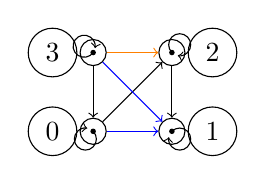
\begin{tikzpicture}
			\path[fill] (0,0)  node[circle] (0) {} node[left=2mm] {0} circle (1pt);
			\path[fill] (1,0)  node[circle] (1) {} node[right=2mm] {1} circle (1pt);
			\path[fill] (1,1)  node[circle] (2) {} node[right=2mm] {2} circle (1pt);
			\path[fill] (0,1)  node[circle] (3) {} node[left=2mm] {3} circle (1pt);

			\path[->,draw] (0) arc(45:-280:1.4mm);
			\path[->,draw] (1) arc(135:-190:1.4mm);
			\path[->,draw] (2) arc(225:-100:1.4mm);
			\path[->,draw] (3) arc(325:-10:1.4mm);
			\path[->,draw] (3) -- (0);
			\path[->,draw] (0) -- (2);
			\path[->,draw] (2) -- (1);
			\visible<2->{\path[->,draw,orange] (3) -- (2);}
			\visible<6->{\path[->,draw,blue] (3) -- (1);}
			\visible<6->{\path[->,draw,blue] (0) -- (1);}
		\end{tikzpicture}
	\column{.4\textwidth}
		\[
		{\color{orange} \sigma^{(0)}}:\
		\alt<2->{
			\left(
			\begin{matrix}
			1 & 0 & 1 & 0\\
			0 & 1 & 0 & 0\\
			0 & 1 & 1 & 0\\
			1 & 0 & {\color{orange}1} & 1
			\end{matrix}
			\right)
		}{
			\left(
			\begin{matrix}
			1 & 0 & 1 & 0\\
			0 & 1 & 0 & 0\\
			0 & 1 & 1 & 0\\
			1 & 0 & 0 & 1
			\end{matrix}
			\right)
		}
		\]
		\[
		\visible<5->{
			{ \color{blue} \sigma^{(2)}}:\
		}
		\alt<-5>{
			\visible<5->{
				\left(
				\begin{matrix}
				1 & 0 & 1 & 0\\
				0 & 1 & 0 & 0\\
				0 & 1 & 1 & 0\\
				1 & 0 & {\color{orange}1} & 1
				\end{matrix}
				\right)
			}
		}
		{
			\left(
			\begin{matrix}
			1 & {\color{blue} 1} & 1 & 0\\
			0 & 1 & 0 & 0\\
			0 & 1 & 1 & 0\\
			1 & {\color{blue} 1} & {\color{orange}1} & 1
			\end{matrix}
			\right)
		}
		\]
	\column{.4\textwidth}
		\[
		\visible<3->{
			{ \color{green} \sigma^{(1)}}:\
		}
		\alt<-3>{
			\visible<3->{
				\left(
				\begin{matrix}
				1 & 0 & 1 & 0\\
				0 & 1 & 0 & 0\\
				0 & 1 & 1 & 0\\
				1 & 0 & {\color{orange}1} & 1
				\end{matrix}
				\right)
			}
		}
		{
			\left(
			\begin{matrix}
			1 & 0 & 1 & 0\\
			0 & 1 & 0 & 0\\
			0 & 1 & 1 & 0\\
			1 & 0 & {\color{orange}1} & 1
			\end{matrix}
			\right)
		}
		\]
		\[
		\visible<7->{
			{ \color{red} \sigma^{(3)}}:\
		}
		\alt<-7>{
			\visible<7->{
				\left(
				\begin{matrix}
				1 & {\color{blue} 1} & 1 & 0\\
				0 & 1 & 0 & 0\\
				0 & 1 & 1 & 0\\
				1 & {\color{blue} 1} & {\color{orange}1} & 1
				\end{matrix}
				\right)
			}
		}
		{
			\left(
			\begin{matrix}
			1 & {\color{blue} 1} & 1 & 0\\
			0 & 1 & 0 & 0\\
			0 & 1 & 1 & 0\\
			1 & {\color{blue} 1} & {\color{orange}1} & 1
			\end{matrix}
			\right)
		}
		\]
	\end{columns}
\end{frame}


\begin{frame}[fragile]
	\frametitle{Der Warshall-Algorithmus}

	\begin{block}{Anforderungsbeschreibung}
		\begin{description}
			\item[Eingabe:]Adjazenzmatrix $A$ einer Relation $\sigma$
			\item[Ausgabe:] Adjanzenzmatrix $S$ von $\sigma^*$ \pause (entspricht der
			Erreichbarkeitsrelation)
		\end{description}
	\end{block}

	\pause
	\begin{block}{Der Algorithmus}
		\begin{lstlisting}[language = Java,mathescape,morekeywords={set}]
	$S$ := $A$
 for $i=0,\ldots,n-1$ set $s_{ii}$ := $1$

 for $k=0,\ldots,n-1$
   for $i=0,\ldots, n-1$
     for $j=0,\ldots, n-1$
       if ($s_{ij}$ + $s_{ik}$ * $s_{kj}$) >= 1 set $s_{ij}$ := 1
		\end{lstlisting}
	\end{block}
\end{frame}


%%%%%%%%%%%%%%%%%%%%%%%%%%%%%%%%%%%%%%%%%%%%%%%%%%%%%%%%%%%%%%%%%%%neu

\section[Effizienz]{Algorithmen-Effizienz}
\subsection*{}
\begin{frame}
  \frametitle{Effizienzberechnung}

  \begin{block}{Problem}
    \begin{itemize}
      \item Ist ein Algorithmus besser als ein anderer?
      \item Gilt das auch auf einer anderen Rechenmaschine?
      \item Gilt es auch, wenn die Datenmenge weiter wächst?
    \end{itemize}
  \end{block}
\pause
  \begin{block}{Lösungsansatz}
    Wir abstrahieren die Effizienz von Algorithmen:
    \begin{itemize}
      \item unabhängig von der Rechenmaschine
      \item in Abhängigkeit der Eingabelänge (meist $n$)
      \item mathematisch fundiert und beweisbar
    \end{itemize}
    So kann anhand der oberen Schranke
				eines Algorithmus z.B. gesagt werden, dass er im schlimmsten Fall (Worst-Case) signifikant langsamer ist,
				als ein anderer.
  \end{block}
\end{frame}


\subsection*{}
\begin{frame}
  \frametitle{$O$-Kalkül}
    \begin{block}{Definition}
          $O(g(n))=\{f(n)| \exists c > 0 \ \exists n_{0} \in \mathbb{N}\ \forall n \ge n_{0}: 0 \le f(n) \le c\cdot g(n)\}$
    \end{block}

    \begin{block}{Umgangssprachlich}
        $O(g(n))$ enthält alle nicht-negativen Funktionen, die höchstens so schnell wie $g(n)$ wachsen.

        Dabei kümmern wir uns nicht

  \begin{itemize}
    \item darum, was am Anfang passiert ($\exists n_0\in\mathbb{N}$ \ldots $\forall n\ge n_0$).
    \item um einfache Faktoren ($\exists c\in\mathbb{R}$ \ldots $c\cdot g(n)$).
  \end{itemize}
  \end{block}
\end{frame}

\subsection*{}
\begin{frame}
  \frametitle{$O$-Kalkül}
    \begin{center}
			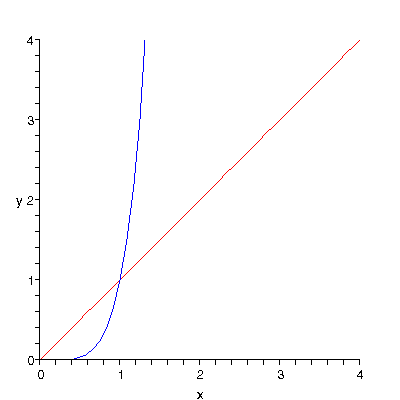
\includegraphics[height=6.2cm]{src/tut08_okalk.png} %[height=5cm]
		\end{center}
\end{frame}

\subsection*{}
\begin{frame}
  \frametitle{Rechnen mit dem $O$-Kalkül}

\begin{small}  Man kann aus der obigen Definition ein paar Regeln ableiten, mit denen der Umgang deutlich einfacher wird.\\
  (Eigentlich rechnet man hier mit Mengen, und auch sonst ist die Schreibweise nicht mathematisch
  korrekt, aber das wird meistens unter den Teppich gekehrt.)\end{small}

  \begin{block}{Faustregeln}
    \begin{itemize}%
      \item $O(1) + O(23) + O(4) = O(1)$
      \item $O( f(n) ) + O( f(n) ) = O( f(n) )$
      \item $O( a\cdot f(n) ) = O(f(n)) \ \forall a\in\mathbb{R}$
      \item $O( a\cdot n^2+b\cdot n+c ) = O( n^2 ) \ \forall a,b,c\in\mathbb{R}$
    \end{itemize}

    \begin{center}"`Der Stärkere gewinnt!"'\end{center}
  \end{block}
\end{frame}

\subsection*{}
\begin{frame}
  \frametitle{Logarithmen}
    \begin{block}{Achtung!}
  		Logarithmen haben alle asymptotisch das gleiche Wachstum: \pause
  \begin{itemize}
  	\item z.z.: $\log_2(n) \in\Theta(\log_8(n))$ \pause
	\item $n = 8^{\log_8 n} = (2^3)^{\log_8(n)} = 2^{3\log_8(n)}$,
		also gilt für alle $n\geq 1$: $\log_2(n) = 3 \log_8(n)$ und $\log_8(n)=\frac{1}{3}\log_2(n)$
	\item allgemein: \pause

 	 $\log_b(n) \in\Theta(\log_a(n))$, denn
	    \[
	    b^{\log_b(n)} = n = a^{\log_a(n)} = (b^{\log_b(a)})^{\log_a(n)} = b^{\log_b(a) \cdot \log_a(n) }
	    \]  \pause
	     $\log_b(n) = \log_b(a) \cdot \log_a(n)$ \\
	    also für $c'=c=\log_b(a)$ und alle $n\geq 1$ gilt: $c \log_a(n) \leq\log_b(n) \leq c' \log_a(n) $ \pause
	 \item Man kann also einfach $\Theta(\log n)$ ohne Basis schreiben
  \end{itemize}
  \end{block}
\end{frame}

\subsection*{}
\begin{frame}
  \frametitle{Berechnung von Potenzen}

  \footnotesize
  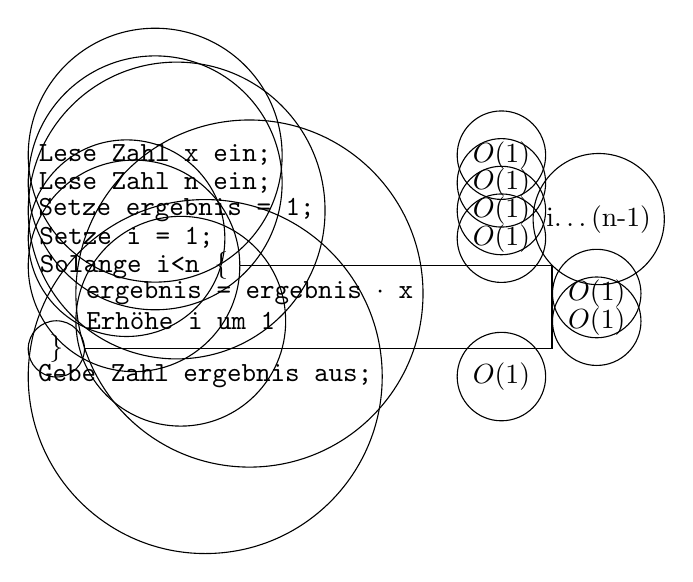
\begin{tikzpicture}[y=1em,x=4ex]
    \node      at (  0,   0)[right] {\texttt{Lese Zahl x ein;}};
    \node      at (  0,   -1)[right] {\texttt{Lese Zahl n ein;}};
    \node      at (  0,   -2)[right] {\texttt{Setze ergebnis = 1;}};
    \node      at (  0,   -3)[right] {\texttt{Setze i = 1;}};

    \node (s1) at (  0,  -4)[right] {\texttt{Solange i<n \{}};
    \node      at (  1,  -5)[right] {\texttt{ergebnis = ergebnis $\cdot$ x}};
    \node 		 at (  1,  -6)[right] {\texttt{Erhöhe i um 1 }};
    \node (s2) at (  0,  -7)[right] {\texttt{\}}};

    \node      at (  0,  -8)[right] {\texttt{Gebe Zahl ergebnis aus;}};

    \visible<2->{\node      at ( 9,  0)[right] {$O(1)$};}
    \visible<3->{\node      at ( 9,  -1)[right] {$O(1)$};}
    \visible<4->{\node      at ( 9,  -2)[right] {$O(1)$};}
    \visible<5->{\node      at ( 9,  -3)[right] {$O(1)$};}
    \visible<6->{ \draw [-] (s1) -| (11,-4) node [above right] {i\ldots(n-1)} |- (s2);}
    \visible<7->{\node      at ( 11,  -5)[right] {$O(1)$};}
    \visible<7->{\node      at ( 11,  -6)[right] {$O(1)$};}
    \visible<8->{\node      at ( 9,  -8)[right] {$O(1)$};}

  \end{tikzpicture}

  \visible<9->{ $$ O(1+1+1+1+ \sum_{i=0}^{n-1}2+1) $$ }
  \visible<9->{$$ =O(n) $$}
\end{frame}


\subsection*{}
\begin{frame}
  \frametitle{Suchen in einer aufsteigend sortierten Liste}

  \footnotesize
  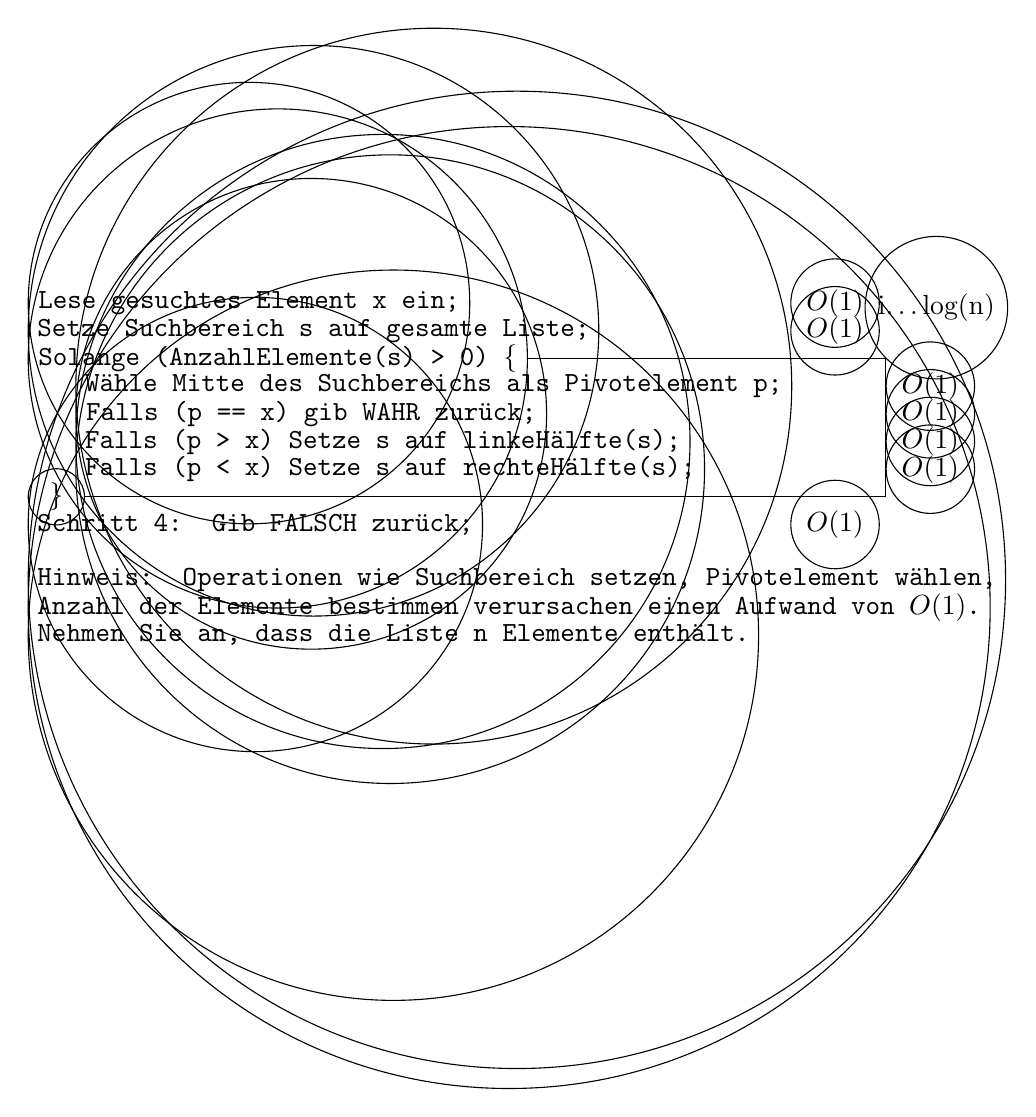
\begin{tikzpicture}[y=1em,x=4ex]
    \node      at (  0,   0)[right] {\texttt{Lese gesuchtes Element x ein;}};
    \node      at (  0,   -1)[right] {\texttt{Setze Suchbereich s auf gesamte Liste;}};

    \node (s1) at (  0,  -2)[right] {\texttt{Solange (AnzahlElemente(s) > 0) \{}};
    \node      at (  1,  -3)[right] {\texttt{Wähle Mitte des Suchbereichs als Pivotelement p;}};
    \node 		 at (  1,  -4)[right] {\texttt{Falls (p == x) gib WAHR zurück;}};
    \node 		 at (  1,  -5)[right] {\texttt{Falls (p > x) Setze s auf linkeHälfte(s);}};
    \node 		 at (  1,  -6)[right] {\texttt{Falls (p < x) Setze s auf rechteHälfte(s);}};
    \node (s2) at (  0,  -7)[right] {\texttt{\}}};

    \node      at (  0,  -8)[right] {\texttt{Schritt 4: Gib FALSCH zurück;}};

    \only<1>{
    	\node      at (  0,  -10)[right]{\texttt{Hinweis: Operationen wie Suchbereich setzen, Pivotelement wählen, }};
    	\node      at (  0,  -11)[right]{\texttt{Anzahl der Elemente bestimmen verursachen einen Aufwand von $O(1)$.}};
    	\node      at (  0,  -12)[right]{\texttt{Nehmen Sie an, dass die Liste n Elemente enthält.}};}

		\visible<2->{\node      at ( 16,  0)[right] {$O(1)$};}
    \visible<3->{\node      at ( 16,  -1)[right] {$O(1)$};}
    \visible<4->{ \draw [-] (s1) -| (18,-2) node [above right] {i\ldots log(n)} |- (s2);}
    \visible<5->{\node      at ( 18,  -3)[right] {$O(1)$};}
    \visible<5->{\node      at ( 18,  -4)[right] {$O(1)$};}
    \visible<5->{\node      at ( 18,  -5)[right] {$O(1)$};}
    \visible<5->{\node      at ( 18,  -6)[right] {$O(1)$};}
    \visible<6->{\node      at ( 16,  -8)[right] {$O(1)$};}

  \end{tikzpicture}

  \visible<7->{ $$ O(1) + O(1) + O(log(n)) + O(1) $$ }
  \visible<7->{$$ =O(log(n)) $$}
\end{frame}


\begin{frame}
			\frametitle{Aufwandsklassen}
			\begin{block}{Fallunterscheidung: Aufwandsklassen}
                \begin{description}
                    \item[$O$-Kalkül] Obere Schranke, die der Algorithmus erreichen, aber nicht überschreiten kann
                    \item[$\Omega$-Kalkül] Untere Schranke und ein "'Mindestaufwand"', den der Algorithmus hat
					\item[$\Theta$-Kalkül] Vereinigung der Betrachtung aus $\Omega(n)$ und $O(n)$.\\
						Es entsteht eine Art Funktionsbereich, den der Algorithmus nie verlässt.
                \end{description}
			\end{block}
\end{frame}


\begin{frame}
			\frametitle{Aufwandsklassen}
		\only<1>{
				Obere asymptotische Schranke\\
				$O(g(n)) = \{f(n) \,|$\\$ \exists c \in \mathbb{R}^+, n_0 \in \mathbb{N} \,\forall n > n_0 : 0 \leq f (n) \leq c \cdot g(n)\}$\\
\vspace{3ex}
				Untere asymptotische Schranke\\
				$\Omega(g(n)) = \{f (n) \,|$\\$ \exists c \in \mathbb{R}^+, n_0 \in \mathbb{N} \,\forall n > n_0 : 0 \leq c \cdot g(n) \leq f (n)\}$\\
\vspace{3ex}
				Asymptotisch scharfe Schranke\\
				$\Theta(g(n)) = \{f (n) \,|$\\$ \exists c_1, c_2 \in \mathbb{R}^+, n_0 \in \mathbb{N} \,\forall n > n_0 :
					0 \leq c_1 \cdot g(n) \leq f (n) \leq c_2 \cdot g(n)\}$\\
		}
		\begin{block}{\bf Beachte:}
		Alle Kalküle geben eine {\bf Menge} von Funktionen an. $f(n) = O(n^2)$ bedeutet also eigentlich $f(n) \in O(n^2)$!
		\end{block}
\end{frame}

\begin{frame}
			\frametitle{Rechenregeln}
			\begin{block}{Reflexivität}
                \begin{itemize}
                    \item $f(n) \in O(f(n))$
                    \item $g(n) \in \Omega(g(n))$
					\item $h(n) \in \Theta(h(n))$
                \end{itemize}
			\end{block}
			\begin{block}{Symmetrie}
					Hier gilt nur:  $f(n) \in \Theta(g(n)) \Leftrightarrow g(n) \in \Theta(f(n))$
			\end{block}
			\begin{block}{asymptotisches Wachstum}
				\begin{itemize}
                    \item $O(n^2 + n + log(n)) = O(n^2)$
                    \item $\Omega(n^2 + n + log(n)) = \Omega(n^2) \subset \Omega(log(n))$
                \end{itemize}
			\end{block}
\end{frame}

\begin{frame}
			\frametitle{Beispiel}
		\begin{block}{\bf Warum gilt...?}
		$O(f(n)) \cdot O(g(n)) = O(f(n) \cdot g(n)) $
		\end{block}
		\begin{description}
			\item[] 			$O(f(n)) \cdot O(g(n))$
			\scriptsize
			\item[$\Rightarrow$] $(\forall h_1(n) \in O(f(n)) \exists c_1, n_0 \in \mathbb{N} \,\forall n > n_0 : 0 \leq h_1(n) \leq c_1 \cdot f(n) ) \wedge $\\
								$(\forall h_2(n) \in O(g(n)) \exists c_2, n_0 \in \mathbb{N} \,\forall n > n_0 : 0 \leq h_2(n) \leq c_2 \cdot g(n) )$
			\normalsize
			\item[$\Rightarrow$] $\forall h_1(n)\cdot h_2(n)  \exists c_3 = c_1 \cdot c_2, n_0 \in \mathbb{N} \,\forall n > n_0 :$\\
								 $ 0 \leq h_1(n) \cdot h_2(n) \leq c_3 \cdot f(n) \cdot g(n)$
			\item[=]			$O(f(n) \cdot g(n))$
		\end{description}
\end{frame}

\begin{frame}
			\frametitle{Wunschbeispiel}
		\begin{block}{\bf Warum gilt...?}
		$ n^2 + n \in O(n^2) $
		\end{block}
		\begin{description}
			\item[] $n^2 + n \in O(n^2)$
			\scriptsize
			\item[$\Leftrightarrow$] $ \exists c \in \mathbb{R}^+, n_0 \in \mathbb{N} \,\forall n > n_0 : 0 \leq n^2+n \leq c \cdot n^2 $
			\normalsize
			\item[Vermutung:] $ c = 2, n_0 = 2$
			\item[Induktionsanfang:] $n=2$ : $ 0 \leq n^2+n = 2^2+2 = 6 \leq 8 = 2 \cdot 2^2 = 2n^2$
			\item[Induktionsvoraussetzung:] $0 \leq n^2+n \leq 2n^2$
			\item[Induktionsschluss] $n \rightarrow n+1$ :\\ $ 0 \leq (n+1)^2 + (n+1) = n^2 + 3n + 2 \leq 2n^2 + 4n + 2 = 2(n+1)^2$ qed.
		\end{description}
\end{frame}

% --- von MichaelR ------------------------------------------------------------

\begin{frame}
	\frametitle{Aufgaben}

	\begin{itemize}
		\item 	Welche Funktionen gehören in welche Klassen?
	\end{itemize}

	\begin{Large}
	\begin{center}
	\begin{tabular}{l|c|c|c|c}
			  & $O(n^2)$ & $\Omega(n^2)$ & $O(\log{n})$ & $\Theta(n)$\\ \hline
	$n^2 + n$	  & \xj & \xj & \xn & \xn \\ \hline
	$n \cdot \log(n)$ & \xj & \xn & \xn & \xn \\ \hline
	$2 \cdot n + 1$	  & \xj & \xn & \xn & \xj \\ \hline
	$n^3$		  & \xn & \xj & \xn & \xn \\ \hline
	$5$		  & \xj & \xn & \xj & \xn
	\end{tabular}
	\end{center}
	\end{Large}

\end{frame}

\section{Abschluss}
% Studis anzuregen darüber nachzudenken, ob sie wirklich alles wissen, ansonsten nachlesen oder fragen nachträglich stellen, dann kann in der nächsten Woche nochmal drauf eingegangen werden
\subsection*{}
\begin{frame}
	\frametitle{Zum Schluss...}
	\begin{block}{Was ihr nun wissen solltet!}
	\begin{itemize}
	  	\visible<2->{\item Wie sind die $O$, $\Omega$ und $\Theta$ Kalküle definiert?}
		\visible<3->{\item Wozu braucht man sie überhaupt?}
		\visible<4->{\item Welche Schreibweise sollten wir verwenden?} %($f\in O(g)$!)
		\visible<5->{\item Was ist eine geschlossene Formel zu einer Rekursion?}
		\visible<6->{\item Was ist eine monoton steigende Funktion?}
    \end{itemize}
   	\end{block}

	\visible<7->{
	\begin{block}{Ihr wisst was nicht?}
		Stellt \textbf{jetzt} Fragen!
	\end{block}}
\end{frame}
